% ----------------------------------------------------------------------------------------------------- %
% Capítulo 3 - FUNDAMENTAÇÃO TEÓRICA
% ----------------------------------------------------------------------------------------------------- %
\chapter{Fundamentação Teórica}
\label{cap:teoria}

\noindent Ao longo desse capítulo serão expostos conceitos básicos que são de grande importância para o entendimento desse trabalho e dentre eles serão destacados a definição de matriz e uma explanação sobre as principais utilizadas no estudo da Álgebra Linear, sistemas de equações lineares que são uns dos conteúdos que farão parte da plataforma de ensino e aprendizagem AlfaGebra, espaço vetorial que também compõe o AlfaGebra, abordagem sobre engenharia de \textit{software} a fim de explanar como consiste o desenvolvimento de um sistema, e para um desenvolvimento mais enxuto a utilização da metodologia ágil \textit{Scrum} que será aplicada no desenvolvimento do \textit{software} AlfaGebra e assim entender seu funcionamento. E por fim, uma abordagem sobre avaliação do ensino e aprendizagem.

\section{Matrizes}
\noindent Um das ferramentas mais poderosas consideradas na matemática são as matrizes, pois as mesmas tem aplicações em diversas áreas, tais como em codificação e decodificação de mensagens, computação gráfica, engenharias, etc. Desse modo, faz-se necessário a compreensão de algumas propriedades e nomenclaturas em relação as mesmas.

\subsection{Definição de matriz}
\noindent Matrizes são objetos matemáticos estruturados em um quadrado composto por linhas e colunas. A definição de Steinbruch \cite{1987:Steinbruch} é similar a citada, onde uma matriz é um quadrado $m x n$ de elementos, e que estes podem ser números, polinômios, funções, etc., que estão dispostos em $m$ linhas e $n$ colunas, representada por  $A{}_{mxn}$.\\

\begin{center}
    $A = 
    \begin{bmatrix}
        a_{11} & a_{12} & a_{13} & \ldots & a_{1n}\\ 
        a_{21} & a_{22} & a_{23} & \ldots & a_{2n}\\ 
        a_{31} & a_{32} & a_{33} & \ldots & a_{3n}\\ 
        \vdots & \vdots & \vdots & \ldots & \\ 
        a_{m1} & a_{m2} & a_{m3} & \ldots & a_{mn}
    \end{bmatrix}_{mxn}$
\end{center}

%
\subsection{Tipos de matrizes}
\noindent Para Boldrini \cite{1980:Boldrini}, no processo de utilização de matrizes, percebe-se que existem algumas que são diferentes, seja pela quantitativo de linhas ou colunas, bem como também pela natureza de seus elementos, a qual apresentam propriedades que se diferenciam de uma matriz qualquer. A seguir, serão expostas as principais categorias de matrizes, para isso, considerando uma matriz com $m$ linhas e $n$ colunas representa por $A{}_{mxn}$.

\subsubsection{Matriz Quadrada}
\noindent Quando o número de linhas $m$ é igual ao número de coluna $n$ $(m = n)$.

\textit{Exemplo:}
\begin{center}
    $A = 
    \begin{bmatrix}
        a_{11} & a_{12} & a_{13} \\ 
        a_{21} & a_{22} & a_{23} \\ 
        a_{31} & a_{32} & a_{33} 
    \end{bmatrix}_{mxn}$
\end{center}

Observando a matriz $A$, percebe-se que o número de linhas e colunas são iguais, sendo $A{}_{3x3}$. Nesse tipo de matriz, em que a ordem é $n$ por $n$, costuma dizer que $A$ é uma matriz de ordem $n$.

\subsubsection{Matriz Linha}
\noindent A matriz que apresenta somente uma linha, ou seja, matriz de ordem $1$ por $n$.

\textit{Exemplo:}
\begin{center}
    $A = 
    \begin{bmatrix}
        a_{1} & a_{2} & a_{3} & \ldots & a_{n}
    \end{bmatrix}_{n x 1}$
\end{center}

\subsubsection{Matriz Coluna}
\noindent A matriz que apresenta somente uma coluna, ou seja, matriz de ordem $n$ por $1$.

\textit{Exemplo:}
\begin{center}
    $A = 
    \begin{bmatrix}
        a_{1} \\ 
        a_{2} \\
        a_{3} \\
        \vdots \\
        a_{n} 
    \end{bmatrix}_{1 x n}$
\end{center}

\subsubsection{Matriz Nula}
\noindent A matriz cujos elementos $a{}_{mn}$ são todos nulos.

\textit{Exemplo:}
\begin{center}
    $A = 
    \begin{bmatrix}
        0 & 0 & 0\\ 
        0 & 0 & 0 
    \end{bmatrix}$
\end{center}

\subsubsection{Matriz Diagonal}
\noindent É uma matriz quadrada em que os elementos que não pertencem a diagonal principal são todos nulos, denotada por $A{}_{mn} = 0$, para $m \neq n$.

\textit{Exemplo:}
\begin{center}
    $A = 
    \begin{bmatrix}
        a_{11} & 0 & 0 \\ 
        0 & a_{22} & 0 \\ 
        0 & 0 & a_{33}  
    \end{bmatrix}$
\end{center}

\subsubsection{Matriz Identidade}
\noindent A matriz escalar de qualquer ordem que tem todos os elementos da diagonal principal $a{}_{mm} = 1$ e $a_{mn} = 0$, para todo $m \neq n$. Representada com $I{}_{n}$, ou simplesmente por $I$ é chamada de matriz identidade.

\textit{Exemplo:}
\begin{center}
    $I_{3} = 
    \begin{bmatrix}
        1 & 0 & 0 \\ 
        0 & 1 & 0 \\ 
        0 & 0 & 1  
    \end{bmatrix}$
\end{center}

\subsection{Operações com matrizes}
\noindent Para uma melhor utilização das matrizes é necessário um entendimento sobre as operações aritméticas aplicadas nelas. Assim, a seguir serão demonstradas as três operações que são aplicadas nelas.

\subsubsection{Multiplicação por um escalar}
\noindent De acordo coma definição de Leon \cite{1998:Leon}, se $A$ é uma matriz e $\alpha$ é um escalar, assim $\alpha A$ será a matriz gerada a partir da multiplicação de cada elemento de $A$ por $\alpha$.

\textit{Exemplo:}
\begin{center}
    $5 x
    \begin{bmatrix}
        1 & 3 & 6 \\ 
        -4 & 2 & 0 \\ 
        5 & 7 & -1  
    \end{bmatrix}
    =
    \begin{bmatrix}
        5 \cdot 1 & 5 \cdot 3 & 5 \cdot 6 \\ 
        5 \cdot (-4) & 5 \cdot 2 & 5 \cdot 0 \\ 
        5 \cdot 5 & 5 \cdot 7 & 5 \cdot (-1)  
    \end{bmatrix}
    =
    \begin{bmatrix}
        5 & 15 & 30 \\ 
        -20 & 10 & 0 \\ 
        25 & 35 & -5
    \end{bmatrix}$
\end{center}

Em relação as propriedades da multiplicação de uma matriz por um escalar, para quaisquer matrizes $A$ e $B$ de mesma ordem e os escalares $\alpha$ e $\lambda$ reais a multiplicação por o escalar satisfaz as presentes propriedades:
\begin{enumerate}
    \item[i)] $(\alpha \lambda) A = \alpha(\lambda A)$
    \item[ii)] $(\alpha + \lambda) A = \alpha A + \lambda A$
    \item[iii)] $\alpha(A + B) = \alpha A + \alpha B)$
    \item[iv)] $1 A = A$
\end{enumerate}
 
\subsubsection{Soma de matrizes}
\noindent Dadas duas matrizes $A = (a{}_{mn})$ e $B = (b{}_{mn}) $ são matrizes $m x n$. Assim, a soma $A + B$ é a matriz $m x n$, cujos elementos $(m, n)$ é $(a{}_{mn}) + (b{}_{mn})$, para cada par ordenado $(m, n)$.

\textit{Exemplo:}
\begin{center}
    $A =
    \begin{bmatrix}
        a{}_{11} & a{}_{12} & a{}_{13} \\ 
        a{}_{21} & a{}_{22} & a{}_{23} 
    \end{bmatrix}
    + B =
    \begin{bmatrix}
        b{}_{11} & b{}_{12} & b{}_{13} \\ 
        b{}_{21} & b{}_{22} & b{}_{23}
    \end{bmatrix}
    =
    \begin{bmatrix}
        a{}_{11} + b{}_{11} & a{}_{12} + b{}_{12} & a{}_{13} + b{}_{13} \\ 
        a{}_{21} + b{}_{21} & a{}_{22} + b{}_{12} & a{}_{23} + b{}_{13}
    \end{bmatrix}$
\end{center}

Em relação às propriedades da adição de matrizes, para quaisquer matrizes $A, B$ e $C$ de mesma ordem $m x n$, existem as seguintes propriedades que a satisfazem:

\begin{enumerate}
    \item[i)] $A + (B + C) = (A + B) + C$
    \item[ii)] $A + 0 = 0 + A = A$
    \item[iii)] $-A + A = A - A = 0$
    \item[iv)] $A + B = B + A$
\end{enumerate}

\subsubsection{Multiplicação de matrizes}
\noindent Uma das operações mais importantes é a multiplicação entre matrizes. De acordo com Leon \cite{1998:Leon}, a motivação da definição a seguir de multiplicação entre matrizes vem de sua aplicação em sistemas lineares.

A definição dada por Leon \cite{1998:Leon}, diz que, se $A = (a{}_{mn})$ é uma matriz $m x n$ e  $B = (b{}_{mn)$ é uma matriz $n x r$, assim o produto $AB = C = (c{}_{mn)$ é a matriz $m x r$ cujos elementos são definidos por 

\begin{center}
    $c_{mnj} = \sum_{i}^{k=1}a_{mk}b_{kn}$
\end{center}

Desse modo, para formar o elemento $(m, n)$ do produto, pega-se a \textit{m-ésima} linha de $A$ e a \textit{n-ésima} coluna de $B$, e assim multiplicam-se os elementos correspondentes dois a dois e soma-se os números resultantes. Contudo, para que o produto $AB$ seja possível é necessário que exista se, e somente se, o número de colunas de $A$ seja igual ao número de linhas $B$.

\textit{Exemplo:}
\begin{center}
    $A = 
    \begin{bmatrix}
        1 & 2 & 3 \\ 
        -2 & 1 & 6 
    \end{bmatrix}$
    e $B = 
    \begin{bmatrix}
        3 & -2 \\ 
        2 & 4 \\
        1 & -3 
    \end{bmatrix}$
\end{center}

então:

\begin{center}
    $AB =
    \begin{bmatrix}
        1 \cdot 3 + 2 \cdot 2 + 3 \cdot 1 & 1 \cdot (-2) + 2 \cdot 4 + 3 \cdot (-3) \\ 
        (-2) \cdot 3 + 1 \cdot 2 + 6 \cdot 1 & (-2) \cdot (-2) + 1 \cdot 4 + 6 \cdot (-3)
    \end{bmatrix}
    =
    \begin{bmatrix}
        10 & -3 \\ 
        2 & -10 
    \end{bmatrix}$
\end{center}

\section{Sistemas de Equações Lineares}
\noindent Na matemática, provavelmente um dos problemas considerados mais importantes é a resolução de sistemas de equações lineares. Leon \cite{1998:Leon} destaca a importância desse conteúdo na Álgebra Linear, visto que muitos dos problemas matemáticos que são encontrados em aplicações científicas e industriais abordam em alguma etapa do processo a resolução de um sistema linear. Usando os métodos matemáticos modernos, em muitos dos casos é possível minimizar o problema a um único sistema de equações lineares. E as aplicações e utilização de sistemas de equações lineares está presente em várias áreas como administração, sociologia, economia, ecologia, demografia, engenharia, física, genética, entre outras.

\subsection{Equação Linear}
\noindent Por definição uma equação linear é uma equação da forma: 
\begin{center}
    $a_{1}x_{1} + a_{2}x_{2} + a_{3}x_{} + ... + a_{n}x_{n} = b$   
\end{center}
onde $a_{1}, a_{2}, ..., a_{n}$ são os coeficientes das variáveis, b o termo independente e $x_{1}, x_{2}, x_{3}, ..., x_{n}$ são variáveis.

\subsection{Sistemas de equações lineares}
\noindent Um sistema de equações lineares refere-se a um conjunto de equações do tipo:\\

$\left\{\begin{matrix}
    a_{11}x_{1} + a_{12}x_{2} + a_{13}x_{3} + \ldots + a_{1n}x_{n} = b_{1}\\ 
    a_{21}x_{1} + a_{22}x_{2} + a_{23}x_{3} + \ldots + a_{2n}x_{n} = b_{2}\\ 
    a_{31}x_{1} + a_{32}x_{2} + a_{33}x_{3} + \ldots + a_{3n}x_{n} = b_{3}\\ 
    \ldots\\ 
    a_{m1}x_{1} + a_{m2}x_{2} + a_{m3}x_{3} + \ldots + a_{mn}x_{n} = b_{m}\\ 
\end{matrix}\right$

\subsection{Operações Elementares}
\noindent As operações elementares sobre as linhas de uma matriz são um total de três:
\begin{itemize}
    \item Permutação de duas equações $(Linha_{m} \rightarrow Linha_{n})$:\\
    \textit{Exemplo:}\\
    $Linha_{2} \rightarrow Linha_{3}$
    $\begin{center}
        \begin{bmatrix}
         a & b\\ 
         c & d\\ 
         e &  f
        \end{bmatrix}
        \rightarrow 
        \begin{bmatrix}
         a & b\\ 
         e & f\\ 
         c & d
        \end{bmatrix}\\
    \end{center}$\\
\end{itemize}

\begin{itemize}
    \item Multiplicação de uma equação por um escalar $k$ não nulo $(Linha_{m} \rightarrow k\cdot Linha_{n})$:\\
    \textit{Exemplo:}\\
    $Linha_{2} \rightarrow 2 \cdot Linha_{2}$
    $\begin{center}
        \begin{bmatrix}
         a & b\\ 
         c & d\\ 
         e &  f
        \end{bmatrix}
        \rightarrow 
        \begin{bmatrix}
         a & b\\ 
         2 \cdot c & 2 \cdot d\\ 
         e & f
        \end{bmatrix}\\
    \end{center}$\\
\end{itemize}

\begin{itemize}
    \item Substituição de uma linha por sua soma com outra equação previamente multiplicada por um escalar $k$ não nulo $(Linha_{i} \rightarrow Linha_{m} + k \cdot Linha_{n})$:\\
    \textit{Exemplo:}\\
    $Linha_{2} \rightarrow Linha_{2} + 2 \cdot Linha_{1}$
    $\begin{center}
        \begin{bmatrix}
         a & b\\ 
         c & d\\ 
         e &  f
        \end{bmatrix}
        \rightarrow 
        \begin{bmatrix}
         a & b\\ 
         c+2 \cdot a & d+2 \cdot b\\ 
         e & f
        \end{bmatrix}$\\
    \end{center}
\end{itemize}

\subsection{Forma Escada}
\noindent Por definição dada por Boldrini \cite{1980:Boldrini}, uma matriz de dimensões $m \times n$ é considerada linha reduzida à forma escada se atender aos presentes requisitos abaixo:

\begin{enumerate}
    \item O primeiro elemento de cada linha diferente de zero é igual a 1.
    \item Cada coluna que apresenta o primeiro elemento diferente de zero de alguma linha tem todos os demais elementos iguais a zero.
    \item Se existirem linhas com todos os elementos iguais a zero, elas ficam abaixo de todas as linhas não-nulas.
    \item O número de zeros que preceda o primeiro elemento não nulo, aumenta a cada linha.
\end{enumerate}

\subsubsection{Definição:}
\noindent Dada uma matriz $A_{mxn}$, seja $B_{mxn}$ a matriz linha reduzida à forma escada de $A$. O posto de $A$, denotado por $P$ é a quantidade de linhas não nulas de $B$ e a nulidade de $A$ é o número $n-p$.

\subsection{Soluções de um sistema de equações lineares}
\noindent Dentro da resolução de sistemas de equações lineares podem ocorrer diversas situações na resolução. Considerando um sistema ax = b existirão três possibilidades:
\begin{enumerate}
    \item O sistema possui uma única solução. O sistema nesse caso é dito compatível e determinado ou sistema possível e determinado.
    \item Sistema possui infinitas soluções. O sistema é dito compatível e indeterminado ou sistema possível e indeterminados.
    \item Sistema não possui solução. O sistema é dito incompatível ou impossível. 
\end{enumerate}

\section{Espaço Vetorial}
\noindent Leon \cite{1998:Leon} explana que ``as operações de soma e multiplicação por um escalar são usadas em diversos contextos em matemática. Independentemente do contexto, no entanto, essas operações obedecem, em geral, ao mesmo conjunto de regras aritméticas". E diante de tal, aplicações de sistemas matemáticos que abordam as operações de soma e multiplicação por um escalar apresentam aplicações em várias áreas da matemática e esses sistemas matemáticos desse modelo são chamados de espaços vetoriais. 

Abramo \cite{2016:Abramo} destaca que espaço vetorial está presente em zonas importantes da análise matemática e da geometria diferencial. A utilização de espaços vetoriais está presente em diversas aplicações e áreas, dentre algumas delas, a computação gráfica com sua utilização no espaço espectral de cores, no sistema RGB (\textit{Red, Green e Blue}), em aplicações na física moderna, entre outras.

\subsection{Espaços Vetoriais}
\subsubsection{Definição}
\noindent Boldrini \cite{1980:Boldrini} defini um espaço vetorial real como um conjunto $V$, não vazio, com as seguintes operações: soma, $V\times V\overset{+}{\rightarrow}V$ e a multiplicação por escalar, $\mathbb{R}\times V\overset{\cdot}{\rightarrow}V$ assim, para quaisquer $u, v, w$ e $a, b \in \mathbb{R}$, as propriedades são satisfeitas.

\subsubsection{Operação soma}
\begin{enumerate}
    \item $(u + v) + w = u + ( v + w)$
    \item $u + v = v + u$
    \item Existe $0 \in v$ tal que $0 + v = v$ (0 é chamado vetor nulo)
    \item Existe $- u \in v$ tal que $u + (-u) = 0$
\end{enumerate}
\subsubsection{Operação multiplicação}
\begin{enumerate}
    \item $a(u + v) = au + av$
    \item $(a + b)v = av + bv$
    \item $(ab)v = a(bv)$
    \item $1u = u$
\end{enumerate}

\subsection{Subespaços Vetoriais}
\noindent Em alguns casos é necessário descobrir dentro de um espaço vetorial $V$, subconjuntos $W$ que sejam eles próprios espaços vetoriais menores. Estes conjuntos são chamados de subespaços de $V$. Por exemplo, considerando $V = R^{2}$ o plano onde $W$ é uma reta deste plano, que passa pela origem.

\begin{figure}[!hb]
  \centering 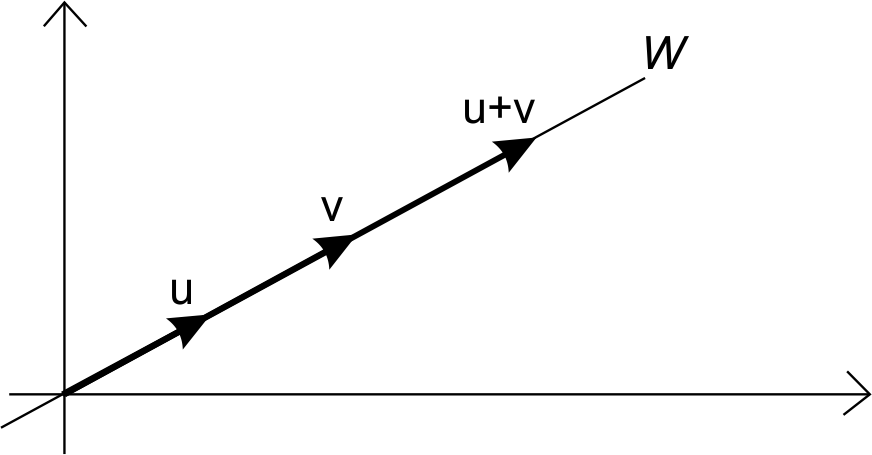
\includegraphics[dimensões]{Figuras/subespacos.png}
  \caption{Subespaço.}
  \label{chave_para_refencia_cruzada}
\end{figure}

\subsubsection{Definição:}
\noindent Dado um espaço vetorial de $V$, um subconjunto $W$, não vazio, será um espaço vetorial de $V$ se atender as duas condições:

\begin{enumerate}
    \item $\forall u, v \in W \rightarrow u + v \in W$
    \item $\forall \alpha \in \mathbb{R}$ e $u \in W \rightarrow \alpha u \in W$
\end{enumerate}

\textit{Exemplo:}\\
Nesse exemplo verifica-se se o conjunto $W = \left \{ (x, 2x) ; x \in \mathbb{R} \right \} \subset \mathbb{R}^2$ é um subespaço vetorial.

Inicialmente deve-se verificar se o vetor nulo está dentro do subespaço assim:
\begin{center}
    $(0, 2\cdot0) = (0,0) \in W$    
\end{center}
Como a verificação é válida, o vetor nulo encontra-se dentro do subespaço, agora analisando as condições da definição:

\subsubsection{Condição 1}
\noindent Sejam $u = (x_{1}, 2x_{1}), v = (x_{2}, 2x_{2}) \in W$. Verificando se $u + v \in W$:
\begin{center}
    $u + v = (x_{1}, 2x_{1}) + (x_{2}, 2x_{2})$\\
    $u + v = (x_{1} + x_{2}, 2x_{1}) + 2x_{2})$\\
    $u + v = (x_{1} + x_{2}, 2(x_{1} + x_{2}) \in W$\\
\end{center}
Observando o resultado obtido percebe-se que a ordenada é o dobro da abscissa.

\subsubsection{Condição 2}
\noindent Sejam $\alpha \in \mathbb{R}$ e $u = (x_{1}, 2x_{1}) \in W$. Verificando se $\alpha u \in W$:
\begin{center}
    $\alpha u = \alpha(x_{1}, 2x_{1})$\\
    $\alpha u = (\alpha x_{1}, \alpha 2x_{1})$\\
    $\alpha u = (\alpha x_{1}, 2(\alpha x_{1})) \in W$\\
\end{center}
Como as duas condições são satisfeitas, então o conjunto é um subespaço vetorial.


\section{Computação simbólica}
\noindent A computação simbólica ou como é conhecida também, computação algébrica, é uma área da computação que trata do estudo e desenvolvimento de algoritmos para manipulação de expressões matemáticas e outros objetos matemáticos. Campos \cite{2015:Lidio} define a computação simbólica como:
\begin{quote}
    um interessante recurso de programação de alto nível, que integra os paradigmas de programação procedural, programação funcional e programação baseada em regras, que permite aos programadores especialistas produzirem aplicações que sistematicamente trabalham o desenvolvimento de Cálculo analítico avançado (p. 4).  
\end{quote}

A computação apresenta limitação  no que tange a capacidade de armazenamento de dados, sua capacidade é limitada, em virtude disto os arredondamentos são aplicados e acabam afetando a precisão da resposta esperada. Mas, a computação simbólica apresenta uma diferencial, pois os dados são armazenados como frações e manipulados algebricamente, o que ocasiona a precisão da resposta total.

A computação simbólica é bastante utilizada na matemática para o desenho de fórmulas que são utilizadas em programas numéricos e esse recurso ajuda a simplificar as tarefas dos usuários ao realizarem cálculos manualmente. Objetiva-se o desenvolvimento do AlfaGebra aplicando os recursos da computação simbólica, pois esse ramo da ciência da computação e da matemática centraliza no estudo de problemas relacionados a objetos não numéricos que podem ser tratados pelo computador, tais como fatoração de polinômios, equações algébricas e equações diferencias, limites, derivadas, integral e operações com matrizes.

\section{\textit{Softwares} matemáticos com abordagem em Álgebra Linear}
\noindent Nesta seção estão apresentados alguns \textit{softwares} com abordagem em Álgebra Linear para resolução de problemas.

\subsection{Matlab}
\noindent Matlab\footnote[1]{Matlab \url{https://www.mathworks.com/products/matlab.html}} é um \textit{software} poderosos, ``conhecido mundialmente como uma excelente ferramenta para soluções de problemas matemáticos, científicos e tecnológicos, que possui comandos muito próximos da forma como são escritas as expressões matemáticas"  (\cite{2005:Marcello}, 2005, p. 2). Sua aplicação é usada para resolução de problemas em diversas áreas, tais como: processamento de imagens, animação, aprendizagem profunda, visão computacional, robótica, etc. \cite{2004:Wu}. Trata-se de um \textit{software} interativo de alta performance voltado para o cálculo numérico, desenvolvido no final dos anos de 1970 pelo o presidente do departamento de ciência da computação da Universidade do Novo México, Cleve Moler.

Uma das principais características presente no Matlab é a sua extensibilidade, que permite que vários contribuintes interajam  para o enriquecimento do sistema, tais como engenheiros, programadores, matemáticos cientistas, entre outros \cite{2005:Marcello}. O sistema aborda uma parte específica para a resolução de problemas voltados para a Álgebra Linear, como sistemas de equações lineares, espaços vetoriais, transformações lineares, entre outros conteúdos e tais recursos facilitam no processo de resolução de problemas.

\subsection{Wolfram Alpha}
\noindent Wolfram Alpha\footnote[2]{Wolfram Alpha \url{https://www.wolfram.com/}} é uma plataforma de conhecimento computacional desenvolvido pela Wolfram Research e é uma plataforma de serviços \textit{online} que responde às perguntas diretamente, mediante o processamento da resposta extraída de base de dados estruturado. O presente sistema realiza cálculos em diversas áreas como cálculo diferencial, processamento de imagens, finanças, Álgebra Linear, entre outros. Através do mesmo é possível obter a resolução problemas mostrando toda a descrição da resolução da expressão.

Na Álgebra Linear, alguns assuntos são abordados para a resolução de problemas, tais como operações com matrizes, sistemas de equações lineares, matrizes de transformações, espaços vetoriais, etc. É importante ressaltar que não são todos os tópicos de sistemas de equações lineares, espaço vetorial e transformações lineares que estão presente na plataforma. 

\subsection{Maple}
\noindent Maple\footnote[3]{Maple \url{https://www.maplesoft.com/}} é \textit{software} computacional específico para resolução de problemas matemáticos e constitui um ambiente computacional para o trabalho com expressões algébricas, simbólica e permite a geração de gráficos em até três dimensões. Seu desenvolvimento começou na Universidade de Waterloo no Canadá em 1981, mas em 1988 a empresa Maplesoft começou a desenvolver novas funcionalidades e a comercializá-lo. 

Com o Maple é possível resolver problemas de diversas áreas, entre elas a Álgebra Linear com a resolução de problemas ligados a sistemas de equações lineares, espaço vetorial, transformações lineares, entre muitos outros tópicos.

\section{Formalismo de linguagens}
\noindent De um modo geral, linguagens formais consiste em modelos matemáticos que permite especificar e reconhecer linguagens, suas estruturas, propriedades e classificações. Em ciência da computação apresenta diversas aplicações tais como modelagem de sistemas, compiladores, processamento de linguagens, reconhecimento de padrões, item este que será de grande importância para o desenvolvimento da plataforma AlfaGebra, pois através do mesmo será possível verificar as expressões inseridas para o processamento do resultado. Contudo, para um melhor entendimento é necessário introduzir os conceitos de alfabeto e palavra.

De acordo com Hopcroft \cite{2002:John}, um alfabeto é um conjunto de símbolos finito e não-vazio e palavra é uma sequência finita de símbolos de um alfabeto, e a partir de um conjunto palavras que são originadas as linguagens.

\subsection{Expressões Regulares}
\noindent Expressões regulares é um notação para definição de padrões para linguagens, sua funcionalidade é para validar entradas de dados, ou seja, é um formalismo denotacional, considerado gerador, o qual é definido a partir de conjuntos de linguagens básicas e de operação de concatenação e de união.

As expressões regulares são utilizadas para construção de muitos \textit{softwares}, por exemplo, compiladores, editores, sistemas operacionais, protocolos, entre outras aplicações e elas são a maneira mais compacta e simples de descrever conjuntos regulares.

\subsection{Autômato Finito}
\noindent Autômato Finito consiste de um formalismo operacional ou reconhecedor, sendo um sistema de estados finitos, ou seja, é uma máquina de estados finito que aceita ou rejeita palavras. De acordo com \cite{2002:John}, 
\begin{quote}
    os autômatos finitos envolvem estados e transições entre estados em reposta a entradas. Eles são úteis na elaboração de vários tipos diferentes de \textit{software}, inclusive o componentes léxica de um compilador e sistemas para verificar correção de circuitos ou protocolos (p. 36).
\end{quote}

Assim como as expressões regulares os autômatos finitos propicia a formalização das linguagens regulares. Contudo, os autômatos finitos são dispositivos de aceitação de sentenças e constituem um caso particular do modelo geral de reconhecedores.

\section{Metodologia de Desenvolvimento Ágil}
\noindent Um ponto importante das metodologias ágeis é que elas são adaptativas, ou seja, elas podem ser adaptadas no decorrer do desenvolvimento de \textit{software} a novos fatores, o que é diferente das metodologias clássicas, a qual pode acontecer de no decorrer do desenvolvimento de um \textit{software} realizar todas as etapas necessárias para sua concretização e depois verificar que elas não atendem mais ao propósito que foi implementado. Isso porque as regras podem ter mudado e para a realização das adaptações pode ter um custo alto, desse modo, não sendo proveitoso desenvolvê-las. Foi a partir dessa situação que a crise do \textit{software} começou a crescer, visto que os \textit{software} não satisfaziam os clientes ou empresas \cite{2005:rezende}.

\subsection{Manifesto Ágil}
\noindent O manifesto ágil teve seu surgimento em 2001 pelo engenheiro de \textit{software} Kenet Beck e mais 16 (dezesseis) desenvolvedores de sistemas de grande destaques na área, a qual batizaram de \textit{``Agile Alliance"} e assinaram um documento conhecido com \textit{``Manifesto para Desenvolvimento Ágil de \textit{Software}"} como registro dessa prática de desenvolvimento \cite{2001:Pressman}.

Atualmente o processo de desenvolvimento de \textit{software} utilizando a metodologia ágil tem ganhado bastante espaços devido ao fato que Pereira \cite{2013:Pereira} relata:
\begin{quote}
    os processos ágeis de desenvolvimento compartilham a premissa de que o cliente aprende sobre as suas necessidades, na medida em que é capaz de manipular o sistema que está sendo produzido e, com base no \textit{feedback} do sistema, ele reavalia as suas necessidades e prioridades, criando mudanças que devem ser incorporadas ao \textit{software} (\cite{2013:Pereira}, apud \cite{2004:Teles}, 2004). 
\end{quote}

\subsection{Metodologia \textit{Scrum}}
\noindent Dentre as metodologias ágeis atualmente presentes no mercado, existe o \textit{Scrum}, esta criada em 1990 por Jeff Sutherland e sua equipe de desenvolvimento, mas somente na década seguinte que se tornou popular. Recentemente Scwaber Beedle foi o responsável por adicionar novas atualizações na metodologia \cite{2001:Pressman}. Tal metodologia aborda todos os princípios utilizados pelo o manifesto ágil, visando a orientação sobre o desenvolvimento de \textit{software} nas atividades de requisitos como levantamento e análise de requisitos, planejamento do projeto, evolução e entrega do produto são atendidos.

O \textit{Scrum} funciona de acordo com seu ciclo de atividades como a figura \ref{chave_para_refencia_cruzada} é demonstrada.

\begin{figure}[!hb]
  \centering 
  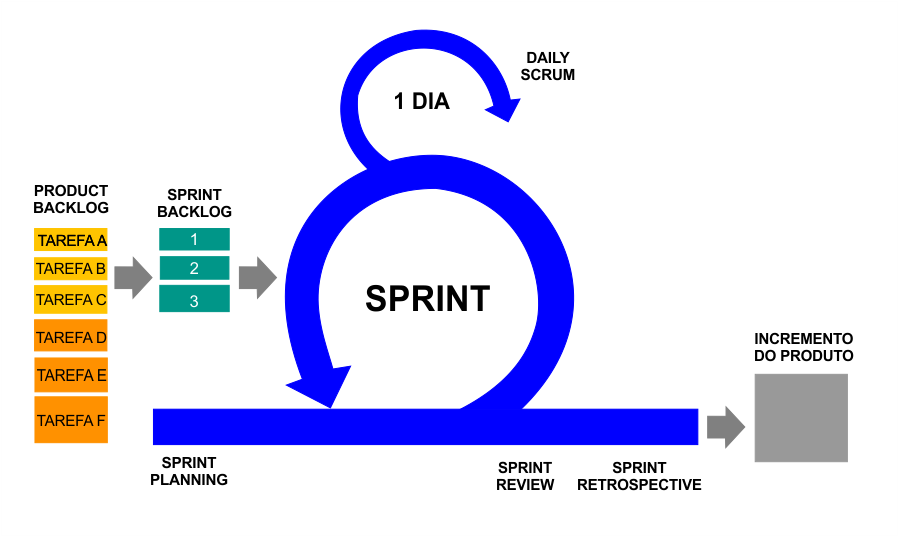
\includegraphics[scale=1.8]{Figuras/ciclo_scrum.png}
  \caption{Ciclo de atividades da metodologia \textit{Scrum}. Adaptado de \cite{0000:rafael}}
  \label{chave_para_refencia_cruzada}
\end{figure}

No decorrer do desenvolvimento vários termos são utilizados para descrever cada etapa, tais como \textit{Product Backlog, Sprint Backlog, Daily Scrum Meeting, Sprint Review Meeting,} entre outras. Adiante serão expostas cada uma com sua importância e significado dentro da metodologia.

\subsubsection{\textit{Product Backlog}}
\noindent O \textit{Product Backlog} consiste em uma lista que nela estarão elencadas tudo que acredita que será produzida ao longo do projeto e os itens presentes nela serão desenvolvidas pelo \textit{Scrum Team}, ou seja, a equipe de desenvolvimento e essa é a única fonte de trabalho que a equipe realiza. E é nela que irão conter todas a necessidades e objetivos de negócio do cliente e as partes interessadas do projeto \cite{0000:rafael}. Essa lista é categorizada com níveis de prioridades e essas prioridades são estabelecidas pelo \textit{Product Owner}.

A figura \ref{chave_para_refencia_cruzada} demonstra como é estruturada a lista de \textit{Product Backlog}, sendo organizada por prioridades. 

\begin{figure}[!htb]
  \centering 
  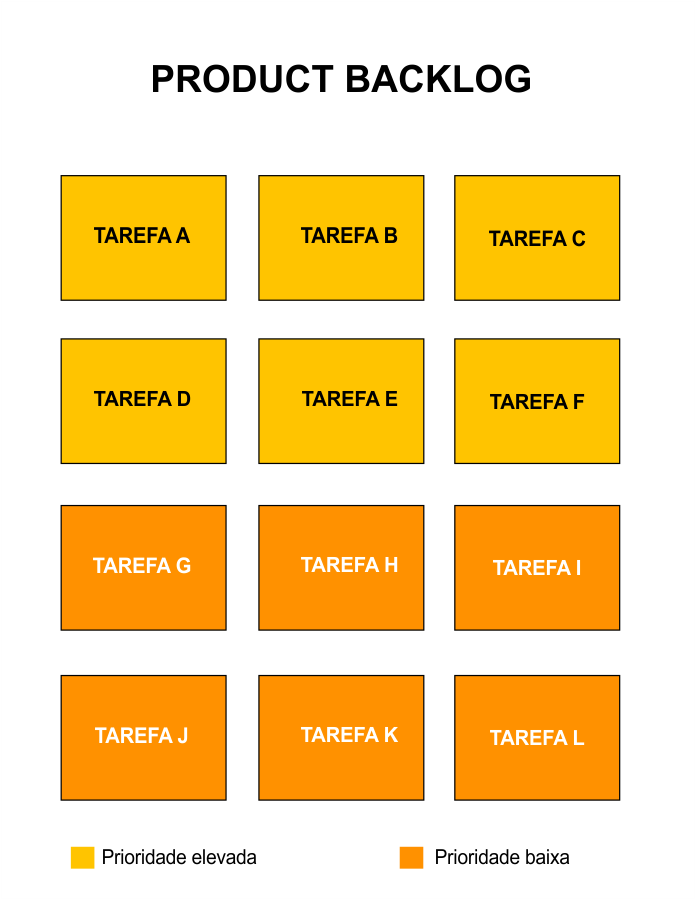
\includegraphics[scale=1.2]{Figuras/product_backlogs.png}
  \caption{Estrutura de um \textit{Product Backlog}. Adaptado de \cite{0000:rafael}}
  \label{chave_para_refencia_cruzada}
\end{figure}

\subsubsection{\textit{Sprint Backlog}}
\noindent Uma \textit{Sprint} de acordo com Kotonya \cite{1997:Kotonya} consiste em um planejamento que visa avaliar a situação do trabalho, os recursos alocados para o desenvolvimento são selecionados e o \textit{software} é implementado. Desse modo, ela é basicamente uma lista que o time de desenvolvimento se compromete a realizar as tarefas presentes. Uma \textit{Sprint} é criada no primeiro evento realizado no ciclo, que é a \textit{Sprint Planning}. Durante a \textit{Sprint} a equipe de desenvolvimento verifica o quadro e solicita a tarefa que acredita que irá conseguir desenvolver e levando em consideração as prioridades de cada.

A figura \ref{chave_para_refencia_cruzada} demonstra a estruturação de um quadro de \textit{Sprint}, sendo que é dividido em tarefas que tem para fazer, as que estão em desenvolvimento e as que já estão feitas.

\begin{figure}[!htb]
  \centering 
  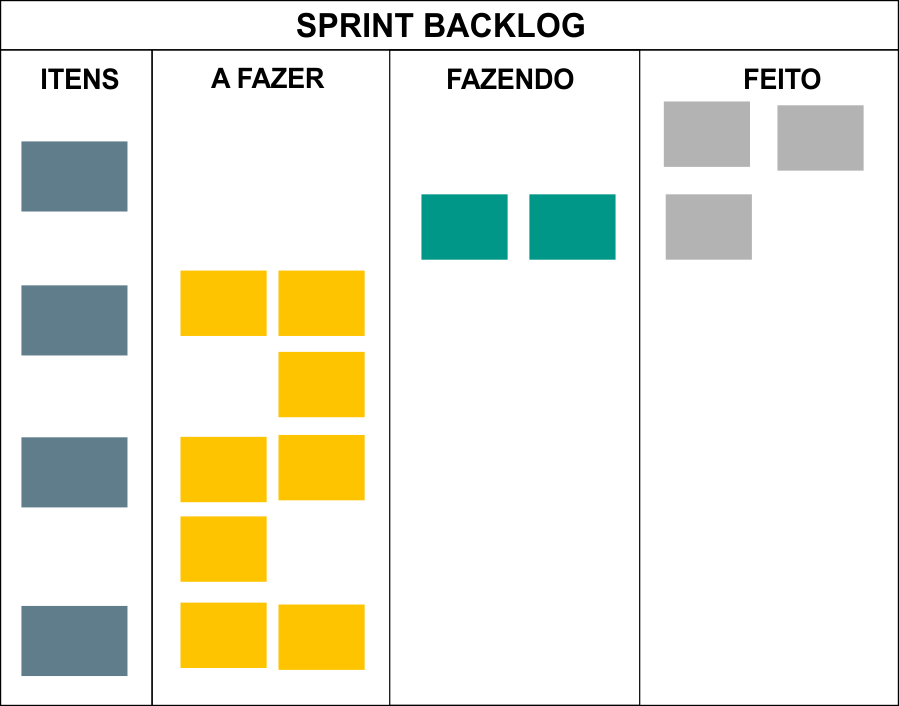
\includegraphics[scale=1.5]{Figuras/sprint_backlog.png}
  \caption{Quadro de tarefas de uma \textit{Sprint Backlog}. Adaptado de \cite{0000:rafael}}
  \label{chave_para_refencia_cruzada}
\end{figure}

\subsubsection{\textit{Daily Scrum Meeting}}
\noindent Todos os dias que os \textit{Sprints} são realizadas a equipe de desenvolvedores, \textit{Product  Owner},\textit{Scrum Master} e outras pessoas, sendo que estas só poderão escutar, participarão de uma reunião que apresenta como objetivo disseminar conhecimentos sobre o que foi realizado no dia anterior e assim conseguir identificar problemas que estão atrapalhando o desenvolvimento e nela são priorizados o trabalho que será realizado no dia.

\subsubsection{\textit{Sprint Review Meeting}}
\noindent Assim como antes de iniciar um \textit{Sprint} é realizado uma reunião para disseminação das informações, no final de cada \textit{Sprint} é realizado também uma reunião que essa apresenta como objetivo de demonstrar o que foi desenvolvido durante o dia, a qual nela participarão toda a equipe, como o \textit{Product Owner, Scrum Team, Scrum Master}, gerência, clientes e engenheiros.

\subsubsection{\textit{Product Owner}}
\noindent Esse é um dos principais personagens da metodologia \textit{Scrum}, pois ele é o responsável por garantir e maximizar o trabalho da equipe, sendo ele que define os itens que irão compor o \textit{Product Baclog}. A partir do momento em que a equipe compromete-se em desenvolver as atividades no \textit{Sprint} ele se compromete a não trazer novos requisitos para \textit{Scrum Team}.

\subsubsection{\textit{Scrum Master}}
\noindent O \textit{Scrum Master} apresenta como função dentro da metodologia de assegurar que a equipe respeite e siga os valores e práticas do \textit{Scrum}, bem como também é o responsável por resolver qualquer impedimento que venha surgir no decorrer da \textit{Sprint}.

\section{Avaliação da aprendizagem}
\noindent A prática de avaliar o aprendizado está presente em todos os momentos da vida acadêmica de um estudante, visto que essa prática faz parte dos objetivos das escolas. E a avaliação de acordo Libâneo \cite{1990:libaneo} não se restringe somente ao processo de realizar provas e atribuir notas, ela é bem mais complexa, pois tem o papel de cumprir as funções pedagógicas-didáticas que se refere ao papel da avaliação seguindo os objetivos gerais e específicos da educação escola, de diagnóstico e de controle em relação aos níveis de rendimento escolar. E esta é uma tarefa necessária e permeante do trabalho do docente. Desse modo, o autor a define como sendo uma reflexão sobre as condições de qualidade do trabalho dos dois personagens principais da academia, os professores e os alunos.

Silva \cite{2015:Silva} apresenta um conceito sobre avaliar parecido com o de Libâneo \cite{1990:libaneo} em que a avaliação não restringe somente no processo de atribuir notas ou conceito para os discentes, mas sim conseguir identificar os espaços que são deixados no decorrer do aprendizado e assim analisar e aplicar estratégias a fim suprir as necessidades identificadas.

Para Datrino \cite{2010:Datrino} na definição de avaliação existem alguns itens que são considerados elementos chaves, sendo eles: julgamento, apreciação, valoração e qualquer efeito que implicar em julgar. Apesar de avaliar implicar medição, a avaliação é algo que é bem mais abrangente do que simplesmente realizar a medição ou qualificação de alguém para saber se adquiriu os conhecimentos.
